\documentclass{beamer}


% Beamer settings
\usecolortheme{rose}
\beamertemplatenavigationsymbolsempty
\setbeamertemplate{footline}[frame number]

\titlegraphic{%

\includegraphics[height=1cm]{logo-full-colour.png}}

\addtobeamertemplate{frametitle}{}{%
\begin{tikzpicture}[remember picture,overlay]
\node[anchor=north east,yshift=2pt] at (current page.north east) {
\includegraphics[height=1cm]{logo-full-colour.png}};
\end{tikzpicture}}

% Packages
\usepackage{amsmath}

\usepackage{tikz}
\usetikzlibrary{positioning}
\usetikzlibrary{fit}

\usepackage{pgfplots}
\usepgfplotslibrary{fillbetween}

\usepackage{minted}
\usepackage[T1]{fontenc} % Required by minted to ensure dollar signs are produced instead of pound (sterling) signs

\usepackage{multicol}

\usepackage{booktabs}

\usepackage{adjustbox}

% Author
\author{Simon McIntosh-Smith \& Tom Deakin\\University of Bristol}

\date{}



\title{OpenMP for Computational Scientists}
\subtitle{5: Programming your GPU with OpenMP}

\begin{document}

\frame{\titlepage}

%-------------------------------------------------------------------------------
\section{Outline}
\begin{frame}
\frametitle{Outline}

\begin{itemize}
  \item Quick recap of NUMA exercise
\end{itemize}

\begin{itemize}
  \item GPU introduction
  \item The OpenMP \mintinline{fortran}|target| construct
  \item Device data environment
  \item Memory movement
  \item Asynchronous offload
  \item Tools
\end{itemize}
\end{frame}

%-------------------------------------------------------------------------------
\section{Recap}
\begin{frame}
\frametitle{Previous exercise}

Take your vectorised 5-point stencil code, with optimised memory access patterns, and consider NUMA issues.
\begin{itemize}
  \item Only one change required: add \mintinline{fortran}|!$omp parallel do| to initilisation loops.
\end{itemize}


Dual-socket Intel Xeon E5-2680 v4 @ 2.40GHz (2x14 cores), Intel 2018, {\tt -O3 -xHost}.
$nx=ny=20,000$, $ntimes=30$. Removed \mintinline{fortran}|write| statement. Taken best of 5 runs.

\begin{table}
\begin{tabular}{ccc}
\toprule
Version & Runtime (s) & Memory bandwidth (GB/s)\\
\midrule
Initial parallel reduction & 25.667 &  7.48 \\
Swap loops + vectorise     &  4.876 & 39.38 \\
NUMA aware initialisation  &  2.365 & 81.18 \\
\bottomrule
\end{tabular}
\end{table}

\end{frame}

%-------------------------------------------------------------------------------
\begin{frame}
\frametitle{Previous exercise}

\begin{itemize}
  \item 81.18~GB/s is 63\% of STREAM Triad bandwidth on this Broadwell system.
  \item This is good! We wouldn't expect to reach Triad bandwidth for more realistic examples.
  \item Missing bandwidth can be explained by looking at vectorisation reports:
  \begin{itemize}
    \item The STREAM kernels use \emph{streaming stores}, and the 5-point stencil doesn't.
  \end{itemize}
\end{itemize}

\end{frame}

%-------------------------------------------------------------------------------
\begin{frame}
\frametitle{Streaming stores}

\begin{itemize}
  \item Streaming stores write directory to main memory, avoiding cache.
  \item Prevents invoking Intel's read-for-ownership mechanism:
  \begin{itemize}
    \item A write to cache required first \emph{reading} the memory (to place it in cache),
    \item and then writing to it.
    \item Doubles the data movement.
  \end{itemize}

\vfill
\pause

  \item STREAM Triad \emph{without} streaming stores gets 94.6~GB/s instead of 129.0~GB/s.
  \item Our kernel can't use streaming stores (alignment): 85.8\% achievable bandwidth.

\vfill
\pause

  \item Much closer! Missing bandwidth may be gained through improving data locality in caches (via tiling).
\end{itemize}

\end{frame}

%-------------------------------------------------------------------------------
\section{GPU introduction}
\begin{frame}
\frametitle{GPU performance}
Why use a GPU?
\begin{itemize}
  \item Hardware trends developing highly parallel processors.
  \item Many simple cores vs few complex cores is one approach.
  \item E.g.: NVIDIA Volta GPUs offer 4.4X memory bandwidth and 1.9X the FLOPS/s of dual-socket Intel Xeon (Skylake).
\end{itemize}


\begin{columns}
\begin{column}{0.5\textwidth}
\begin{adjustbox}{max width={\textwidth}}
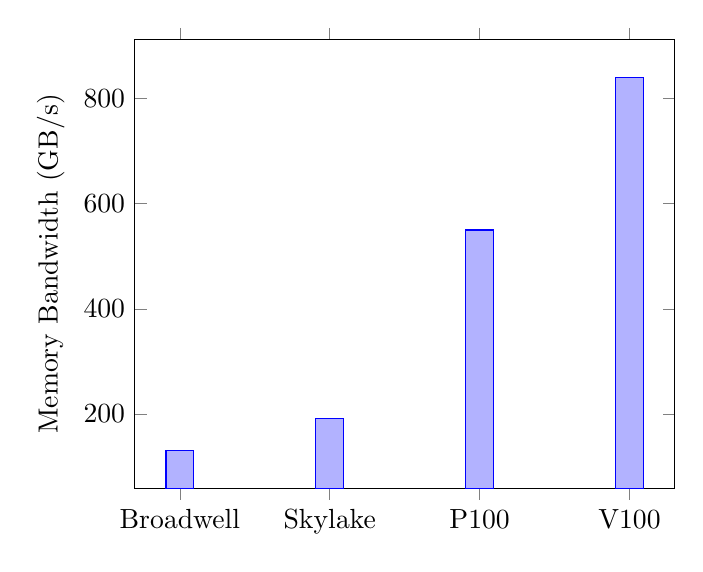
\begin{tikzpicture}
  \begin{axis}[ybar,
               symbolic x coords={Broadwell, Skylake, P100, V100},
               xtick=data,
               ylabel={Memory Bandwidth (GB/s)}]
    \addplot coordinates {(Broadwell,130) (Skylake,191) (P100,550) (V100,841)};
  \end{axis}
\end{tikzpicture}
\end{adjustbox}
\end{column}

\begin{column}{0.5\textwidth}
\begin{adjustbox}{max width={\textwidth}}
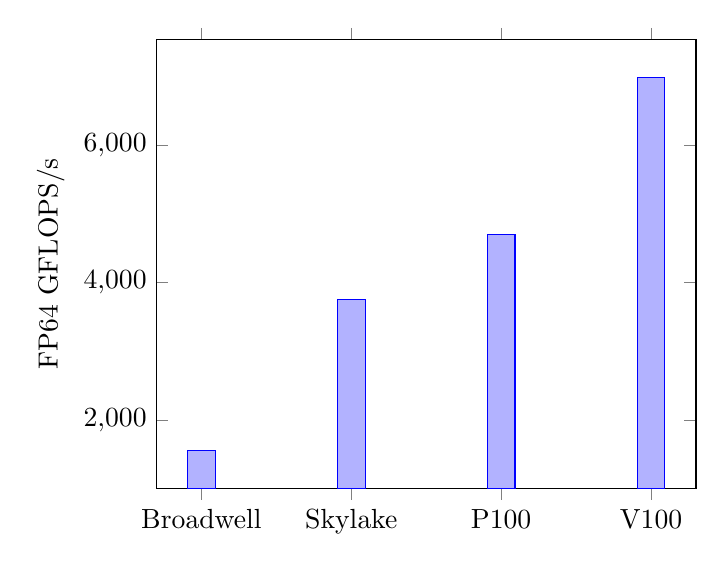
\begin{tikzpicture}
  \begin{axis}[ybar,
               symbolic x coords={Broadwell, Skylake, P100, V100},
               xtick=data,
               ylabel={FP64 GFLOPS/s}]
    \addplot coordinates {(Broadwell,1550) (Skylake,3760) (P100,4700) (V100,7000)};

  \end{axis}
\end{tikzpicture}
\end{adjustbox}
\end{column}
\end{columns}

\end{frame}

%-------------------------------------------------------------------------------
\begin{frame}
\frametitle{Unlocking this potential}
\begin{itemize}
  \item GPUs made of many cores. NVIDIA call them Streaming Multiprocessors (SMs):
    \begin{itemize}
      \item V100 has 80 SMs.
      \item P100 has 56 SMs.
    \end{itemize}
  \item Each SM consists of 64 FP32 CUDA cores.
  \item CUDA cores are really organised as 2 vector units 32 wide (called warps).
\end{itemize}

\begin{block}{Take away}
GPUs are really vector-architectures made up of smaller blocks which execute together.
\end{block}
\end{frame}

%-------------------------------------------------------------------------------
\begin{frame}
\frametitle{GPUs need lots of parallelism}
\begin{itemize}
  \item GPUs are \emph{throughput optimised}, whereas CPUs are \emph{latency optimised}.
  \item Throughput optimised also called \emph{latency tolerant}.
  \item GPUs achieve this by running many operations at once, and overlapping these with each other.
  \item Hence need many (many) operations\dots
  \item A V100 has 5,120 processing elements, each needing multiple units of work to overlap.
\end{itemize}
\begin{block}{Take away}
Massive amounts of parallelism to exploit.
\end{block}
\end{frame}

%-------------------------------------------------------------------------------
\section{OpenMP device model}
\begin{frame}
\frametitle{Device model}
OpenMP has a host/device model.

\begin{center}
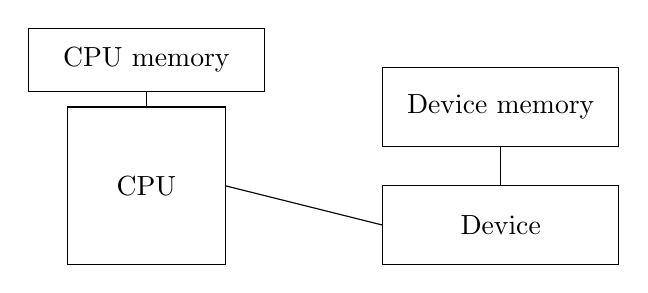
\begin{tikzpicture}

  \draw (0,0) rectangle (2,2);
  \draw (1,1) node {CPU};

  \draw (-0.5, 2.2) rectangle (2.5,3.0);
  \draw (1,2.6) node {CPU memory};
  \draw (1,2) -- (1,2.2);

  \draw (4,0) rectangle (7,1);
  \draw (5.5,0.5) node {Device};

  \draw (4,1.5) rectangle (7,2.5);
  \draw (5.5,2) node {Device memory};
  \draw (5.5,1) -- (5.5,1.5);

  \draw (2,1) -- (4,0.5);


\end{tikzpicture}
\end{center}

\begin{itemize}
  \item Can have more than one device.
  \item Devices are connected to a host CPU via interconnect, such as PCIe or NVLink.
  \item Devices come with their own memory. On NVIDIA HPC GPUs Pascal/Volta this is HBM.
\end{itemize}


\end{frame}
%-------------------------------------------------------------------------------
\begin{frame}[fragile]
\frametitle{Execution model}
\begin{itemize}
  \item Execution begins on the host CPU, with zero or more devices connected to the host.
  \item Memory spaces \emph{not} shared!
  \item In OpenMP, some data copied automatically, plus controls for explicit copying.
  \item Directives are used to transfer execution to the device.
  \begin{minted}{fortran}
  !$omp target [clause [clause] ...]
  !$omp end target
  \end{minted}
  \item Host execution idles until target region completes (exact semantics based on tasks: see next session!).
\end{itemize}

\vfill

\begin{center}
\begin{tikzpicture}
  \draw (-1,0) node {Host};
  \draw (-1,-1) node {Device};
  \draw (0,0) -- (2,0);
  \draw[dashed] (2,0) -- (3,-1);

  % GPU
  \draw (3,-1) -- (5,-1);
  \draw (3,-1.2) -- (5,-1.2);
  \draw (3,-1.4) -- (5,-1.4);
  \draw (3,-1.6) -- (5,-1.6);
  \draw (3,-0.8) -- (5,-0.8);
  \draw (3,-0.6) -- (5,-0.6);
  \draw (3,-0.4) -- (5,-0.4);

  \draw[dashed] (5,-1) -- (6,0);
  \draw[->] (6,0) -- (8,0);
\end{tikzpicture}
\end{center}
\end{frame}

%-------------------------------------------------------------------------------
\begin{frame}
\frametitle{Practically programming a GPU}
\begin{itemize}
  \item Programming the kernels/loops themselves is often the ``easy'' bit!
  \item Most of your programming time will be spent in getting minimal memory movement between host and device.
  \item Performance of the kernels themselves is often good right away assuming you're working with code that was good on a CPU.
  \item Optimisations for memory layout for vectorisation often apply to GPUs.
\end{itemize}

\end{frame}

%-------------------------------------------------------------------------------
\section{Target construct}
\begin{frame}[fragile]
\frametitle{The target construct}

Get code region running on the device.

\begin{minted}{fortran}
!$omp target [clause [clause]...]
  ...
!$omp end target 
\end{minted}
\begin{itemize}
  \item Starts executing \emph{in serial} on the target device.
  \item Need other constructs to expand parallelism.
  \item \mintinline{fortran}|nowait| clause:
    \begin{itemize}
      \item Allows host thread to continue working. Must synchronise later using tasks.
    \end{itemize}
  \item Other clauses mainly about memory movement, which we'll come to later.
\end{itemize}
\end{frame}

%-------------------------------------------------------------------------------
\begin{frame}[fragile]
\frametitle{The one construct you'll need}
In general, you'll run loops on the device using:
\begin{minted}[frame=single]{fortran}
!$omp target teams distribute parallel do
do i = 1, N
  ... ! Loop body
end do
!$omp end target teams distribute parallel do
\end{minted}

\vfill

We'll walk through what the constituent parts mean.

\vfill

\begin{alertblock}{Warning!}
Not using this combined statement can have severe performance issues.
\end{alertblock}
\end{frame}

%-------------------------------------------------------------------------------
\begin{frame}[fragile]
\frametitle{Execution model: teams}

\begin{minted}[frame=single]{fortran}
!$omp target teams 
... ! Code
!$omp end target teams
\end{minted}

\begin{itemize}
  \item OpenMP \emph{threads} on a device are grouped into a \emph{team}.
  \item Can synchronise threads \emph{within} a team.
  \item \emph{Cannot} synchronise between teams (must exit \mintinline{fortran}|target| region for this).
  \item Groups of teams are called a \emph{league}.
  \item \mintinline{fortran}|target| construct offloads (serial) execution to device.
  \item \mintinline{fortran}|teams| construct creates a league of times.
  \item Master thread in \emph{each} team (redundantly) executes the code.
\end{itemize}

\end{frame}

%-------------------------------------------------------------------------------
\begin{frame}
\frametitle{Execution model: teams}
\begin{itemize}
  \item The \mintinline{fortran}|target teams| construct creates a number of teams on the GPU, each containing one thread.
  \item All threads execute code block.
\end{itemize}

\begin{center}
\begin{tikzpicture}
  \draw (0,0) rectangle (1,4);
  \draw[->] (0.5,3.8) -- (0.5,2);

  \draw (2,0) rectangle (3,4);
  \draw[->] (2.5,3.8) -- (2.5,2);

  \draw (4,0) rectangle (5,4);
  \draw[->] (4.5,3.8) -- (4.5,2);

  \draw (6,0) rectangle (7,4);
  \draw[->] (6.5,3.8) -- (6.5,2);
\end{tikzpicture}
\end{center}
\end{frame}

%-------------------------------------------------------------------------------
\begin{frame}[fragile]
\frametitle{Execution model: distribute}
\begin{itemize}
  \item Distribute iterations of a loop across teams.
  \item Each team gets part of the iteration space.
  \item Change default assignment with \mintinline{fortran}|dist_schedule(static)| clause. Optionally include chunk size.
  \item Still only the master thread in the team executes them.
\end{itemize}

\begin{minted}[frame=single]{fortran}
!$omp target teams distribute
do i = 1, N
... ! Code
end do
!$omp end target teams distribute
\end{minted}
\end{frame}

%-------------------------------------------------------------------------------
\begin{frame}
\frametitle{Execution model: distribute}
\begin{itemize}
  \item The \mintinline{fortran}|target teams distribute| construct distributes loop iterations to the teams.
  \item Teams still only contain one thread.
  \item Each team computes a different iteration range.
\end{itemize}

\begin{center}
\begin{tikzpicture}
  \draw (0,0) rectangle (1,4);
  \draw[->] (0.5,3.8) -- (0.5,2);
  \draw (0.5,4.5) node {\mintinline{fortran}|i=1,25|};

  \draw (2,0) rectangle (3,4);
  \draw[->] (2.5,3.8) -- (2.5,2);
  \draw (2.5,4.5) node {\mintinline{fortran}|i=26,50|};

  \draw (4,0) rectangle (5,4);
  \draw[->] (4.5,3.8) -- (4.5,2);
  \draw (4.5,4.5) node {\mintinline{fortran}|i=51,75|};

  \draw (6,0) rectangle (7,4);
  \draw[->] (6.5,3.8) -- (6.5,2);
  \draw (6.5,4.5) node {\mintinline{fortran}|i=76,100|};
\end{tikzpicture}
\end{center}
\end{frame}

%-------------------------------------------------------------------------------
\begin{frame}[fragile]
\frametitle{Execution model: parallel do}
\begin{itemize}
  \item Same semantics as on the CPU!
  \item Launches threads within the team and distributes iterations across those threads.
  \item Note, iterations that were assigned to the team by the \mintinline{fortran}|distribute| construct are distributed across threads in the team.
  \item Can use the \mintinline{fortran}|schedule| clause too.
\end{itemize}

\begin{minted}[frame=single]{fortran}
!$omp target teams distribute parallel do
do i = 1, N
... ! Code
end do
!$omp end target teams distribute parallel do
\end{minted}
\end{frame}

%-------------------------------------------------------------------------------
\begin{frame}
\frametitle{Execution model: parallel do}
\begin{itemize}
  \item The \mintinline{fortran}|target teams distribute parallel do| construct launches threads in each team.
  \item Threads in the team share iteration space assigned by \mintinline{fortran}|distribute| construct.
  \item Finally have lots of parallel execution!
\end{itemize}

\begin{center}
\begin{tikzpicture}
  % Draw teams
  \draw (0,0) rectangle (1,4);
  \draw (2,0) rectangle (3,4);
  \draw (4,0) rectangle (5,4);
  \draw (6,0) rectangle (7,4);

  % Draw 5 threads in each team
  \foreach \j in {0, 2, 4, 6} {
    \foreach \i in {0.1, 0.3, 0.5, 0.7, 0.9} {
      \draw[->] (\j+\i,3.8) -- (\j+\i,2);
    }
  }

  % Label iteration space
  \draw (0.5,4.5) node {\mintinline{fortran}|i=1,25|};
  \draw (2.5,4.5) node {\mintinline{fortran}|i=26,50|};
  \draw (4.5,4.5) node {\mintinline{fortran}|i=51,75|};
  \draw (6.5,4.5) node {\mintinline{fortran}|i=76,100|};

  % Label thread iterations
  \draw (0.5, 1.5) node {\tiny\mintinline{fortran}|0:1,5|};
  \draw (0.5, 1.3) node {\tiny\mintinline{fortran}|1:6,10|};
  \draw (0.5, 1.1) node {\tiny\mintinline{fortran}|2:7,15|};
  \draw (0.5, 0.9) node {\tiny\mintinline{fortran}|3:16,20|};
  \draw (0.5, 0.7) node {\tiny\mintinline{fortran}|4:21,25|};

  \draw (2.5, 1.5) node {\tiny\mintinline{fortran}|0:26,30|};
  \draw (2.5, 1.3) node {\tiny\mintinline{fortran}|1:31,35|};
  \draw (2.5, 1.1) node {\tiny\mintinline{fortran}|2:36,40|};
  \draw (2.5, 0.9) node {\tiny\mintinline{fortran}|3:41,45|};
  \draw (2.5, 0.7) node {\tiny\mintinline{fortran}|4:46,50|};

  \draw (4.5, 1.5) node {\tiny\mintinline{fortran}|0:51,55|};
  \draw (4.5, 1.3) node {\tiny\mintinline{fortran}|1:56,60|};
  \draw (4.5, 1.1) node {\tiny\mintinline{fortran}|2:61,65|};
  \draw (4.5, 0.9) node {\tiny\mintinline{fortran}|3:66,70|};
  \draw (4.5, 0.7) node {\tiny\mintinline{fortran}|4:71,75|};

  \draw (6.5, 1.5) node {\tiny\mintinline{fortran}|0:76,80|};
  \draw (6.5, 1.3) node {\tiny\mintinline{fortran}|1:81,85|};
  \draw (6.5, 1.1) node {\tiny\mintinline{fortran}|2:86,90|};
  \draw (6.5, 0.9) node {\tiny\mintinline{fortran}|3:91,95|};
  \draw (6.5, 0.7) node {\tiny\mintinline{fortran}|4:96,100|};
\end{tikzpicture}
\end{center}
\end{frame}

%-------------------------------------------------------------------------------
\begin{frame}
\frametitle{SIMD construct}
\begin{itemize}
  \item The \mintinline{fortran}|simd| construct is also valid on the \mintinline{fortran}|distribute parallel do| construct.
  \item OpenMP says this means SIMD instructions are generated.
  \item Minor implementation details differ between compilers.
  \item Clang and IBM XL compilers ignore the \mintinline{fortran}|simd| clause.
  \item Cray ignores the \mintinline{fortran}|parallel do| and issues a warning about it, but does a good job of autovectorising.
  \item \mintinline{fortran}|!$omp target teams distribute parallel do| is a portable solution for practically obtaining the same parallelism across compilers.
\end{itemize}


\end{frame}

%-------------------------------------------------------------------------------
\begin{frame}[fragile]
\frametitle{Execution example}

Simple vector addition kernel to illustrate GPU execution.

\begin{minted}[frame=single]{fortran}
!$omp target teams distribute parallel do
do i = 1, N
  c(i) = a(i) + b(i)
end do
!$omp end target teams distribute parallel do
\end{minted}

Might not work out of the box as we haven't said anything about memory movement.

\end{frame}

%-------------------------------------------------------------------------------
\section{Data transfers}
\begin{frame}
\frametitle{Data movement}
\begin{itemize}
  \item Remember: memory is \emph{not} shared between host and target.
  \item OpenMP uses a combination of implicit and explicit memory movement.
  \item This is the most complicated part of the offload specification.

\vfill

  \item Memory movement is often a performance killer.
    \begin{itemize}
      \item A V100 has 900 GB/s peak memory bandwidth.
      \item Connected to the host via PCIe with 32 GB/s peak bandwidth.
      \item Transfers between host and device are relatively very slow: minimise them.
    \end{itemize}
\end{itemize}
\end{frame}

%-------------------------------------------------------------------------------
\begin{frame}[fragile]
\frametitle{Data regions}
\begin{itemize}
  \item Data needs mapping between host and device memory spaces.
  \item Variable names exist in host and device space: the compiler sorts out which one you mean when you use them in your code.
    \begin{minted}{fortran}
      x(i) = 1.0

      !$omp target
      x(i) = 1.0
      !$omp end target
    \end{minted}
  \item OpenMP runtime and compilers must work out when \mintinline{fortran}|x| is in host memory or device memory.
  \item Like having two arrays: \mintinline{fortran}|h_x| and \mintinline{fortran}|d_x| on the host and device respectively.
\end{itemize}
\end{frame}

%-------------------------------------------------------------------------------
\begin{frame}
\frametitle{Data movement}

\begin{itemize}
  \item Mapping/transfers between host and device memory spaces occur when
    \begin{itemize}
      \item enter/exit a \mintinline{fortran}|target| region.
      \item \mintinline{fortran}|target enter/exit data| constructs.
      \item \mintinline{fortran}|update| construct.
    \end{itemize}

\vfill

  \item Default behaviour:
    \begin{itemize}
      \item Scalars are mapped \mintinline{fortran}|firstprivate|.
      \item This means the \emph{do not} get copied back to the host.
      \item Actually saves a memory copy as passed like a subroutine argument.

\vfill

      \item Stack arrays are mapped \mintinline{fortran}|tofrom|.
      \item Heap arrays are not mapped by default.
    \end{itemize}
\end{itemize}
\end{frame}

%-------------------------------------------------------------------------------
\subsection{Map clause}
\begin{frame}[fragile]
\frametitle{The map clause}
\begin{itemize}
  \item Specify the transfer of data between host and device on a \mintinline{fortran}|target| region.

\vfill

  \item Assume we have an array \mintinline{fortran}|A(1:N)| and a scalar \mintinline{fortran}|x|.
  \item Sizes of arrays are generally known in Fortran so don't need to specify amount of data to copy.
  \item Can use array slicing, but slicing whole array buggy with Cray compiler.
  \item (you shouldn't be using assume sized arrays in your kernels anyway!)
\end{itemize}

\begin{minted}[frame=single]{fortran}
!$omp target map(...)
   ...
!$omp end target
\end{minted}

\end{frame}

%-------------------------------------------------------------------------------
\begin{frame}[fragile]
\frametitle{The map clause}
Direction defined from the \emph{host} perspective.
\begin{itemize}
  \item
    \begin{minted}{fortran}
    map(to: A, x)
    \end{minted}
    On entering the region, copy from host to device.

  \item
    \begin{minted}{fortran}
    map(from: A, x)
    \end{minted}
    On exiting the region, copy from device to host. At start of \mintinline{fortran}|target| region, these are uninitialised on the device.

  \item
    \begin{minted}{fortran}
    map(tofrom: A, x)
    \end{minted}
    Same as applying \mintinline{fortran}|map(to: ...)| and \mintinline{fortran}|map(from: ...)|

  \item
    \begin{minted}{fortran}
    map(alloc: A)
    \end{minted}
    Allocate data on the device without copying from the host. It is uninitialised.
    Can later be copied back to the host (with \mintinline{fortran}|update| etc.) as long as allocated on host too.
\end{itemize}
\end{frame}

%-------------------------------------------------------------------------------
\subsection{Enter/exit data constructs}
\begin{frame}[fragile]
\frametitle{Memory movement best practice}

\begin{minted}[frame=single]{fortran}
call initilise(A,B,C)

do t = 1, N
  call update(A)
  call update(B)
  call update(C)
end do
\end{minted}

\begin{itemize}
  \item Scientific codes tend to initialise data at the start, then run many kernels.
  \item Generally don't worry about timing of initialisation.
  \item Poor practice in MPI would for example gather and scatter data to reinitialise data every iteration.
  \item Same applies between host and device memory spaces!
\end{itemize}

\end{frame}

%-------------------------------------------------------------------------------
\begin{frame}[fragile]
\frametitle{Enter/exit data constructs}
\begin{itemize}
  \item Often want to perform initial device data environment setup once, run through iterative loop, copying back at end.
  \item \textbf{Do not} want to copy the data every iteration! Very expensive.
  \item Use \mintinline{fortran}|target enter data| and \mintinline{fortran}|target exit data| constructs to control device data environment.
\end{itemize}

\begin{minted}[frame=single,fontsize=\small]{fortran}
!$omp target enter data map(to: A, B, C)

do t = 1, N
  !$omp target
  ... ! E.g. Read A and B, write C
  !$omp end target
end do

!$omp target exit data map(from: C)

\end{minted}
Bulk transfers happen at beginning and end, not for every \mintinline{fortran}|target| region in the big loop.
\end{frame}

%-------------------------------------------------------------------------------
\begin{frame}[fragile]
\frametitle{Vector addition with memory movement}

\begin{minted}[frame=single,fontsize=\small]{fortran}
! Initialise on host
allocate(A(N), B(N), C(N))
A = 1.0
B = 2.0

! Copy A and B to device, and allocate space for C
!$omp target enter data map(to: A, B) map(alloc: C)

! Run vector add on device
!$omp target teams distribute parallel do
do i = 1, N
  c(i) = a(i) + b(i)
end do
!$omp end target teams distribute parallel do

! Copy C back to host
!$omp target exit data map(from: C)

\end{minted}


\end{frame}

%-------------------------------------------------------------------------------
\subsection{Update}
\begin{frame}
\frametitle{Update construct}
\begin{itemize}
  \item Often need to transfer data between host and device between different \mintinline{fortran}|target| regions.
  \item E.g. the host does something between the two regions.
  \item Example on next slide\dots
  \item Use the \mintinline{fortran}|update| construct to move the data explicitly between host and device, in either direction.
  \item Remember: direction is from the \emph{host's} perspective.
\end{itemize}
\end{frame}

%-------------------------------------------------------------------------------
\begin{frame}[fragile]
\frametitle{Update construct}
\begin{minted}[frame=single,fontsize=\footnotesize,linenos]{fortran}
!$omp target enter data map(to: A, B, C)
!$omp target
... ! Use A, B and C on device
!$omp end target

! Copy A from device to host
!$omp target update from(A(1:N))

! Change A on the host
A = 1.0

! Copy A from host to device
!$omp target update to(A(1:N))

!$omp target
... ! Use A, B and C on device
!$omp end target

!$omp target exit data map(from: C)
\end{minted}

\end{frame}

%-------------------------------------------------------------------------------
\begin{frame}[fragile]
\frametitle{Halo exchange}
Use the \mintinline{fortran}|update| clause with a typical halo exchange pattern.

\begin{minted}[frame=single,linenos,fontsize=\footnotesize]{fortran}
!$omp target enter data map(...)

do t = 1, N
  !$omp target ...
    ... ! run kernel
  !$omp end target ...

  ! Copy latest halo data from device to host
  !$omp target update from(halo)

  ! Exchange with MPI
  call MPI_Sendrecv(halo, ...)

  ! Copy neighbour rank data to device
  !$omp target update to(halo)
end do

!$omp target exit data map(...)
\end{minted}

\end{frame}

%-------------------------------------------------------------------------------
\section{Reductions}
\begin{frame}[fragile]
\frametitle{Reductions}
\begin{minted}[frame=single,breaklines,fontsize=\small]{fortran}
integer :: i, N = 1000
real(kind=8), allocatable :: A(:), B(:)
real(kind=8) :: total

!$omp target map(to: A, B) map(tofrom: total)
!$omp teams distribute parallel do reduction(+:total)
do i = 1, N
  total = total + (A(i) * B(i))
end do
!$omp end teams distribute parallel do
!$omp end target
\end{minted}

\begin{itemize}
  \item \mintinline{fortran}|total| is a scalar, so by default is mapped \mintinline{fortran}|firstprivate|.
  \item I.e. Each thread on the device gets its own copy.
  \item Importantly, it is \emph{not} copied back to the host at the end!
  \item You \emph{must} use a \mintinline{fortran}|map| clause to bring the result back.
\end{itemize}

\end{frame}

%-------------------------------------------------------------------------------
\section{Nowait clause}
\begin{frame}
\frametitle{Asynchronous offload}
\begin{itemize}
  \item By default, the host thread will idle and wait for the \mintinline{fortran}|target| region to complete.
  \item The \mintinline{fortran}|nowait| clause causes the \mintinline{fortran}|target| region to be offloaded as a task.
  \item The host thread can continue working asynchronously with the device!
  \item Must synchronise using \mintinline{fortran}|taskwait|, or at a \mintinline{fortran}|barrier| (explicit or implicit) depending on host threading design.
  \item Uses the OpenMP tasking semantics.
\end{itemize}
\end{frame}

%-------------------------------------------------------------------------------
\begin{frame}[fragile]
\frametitle{Asynchronous offload}
\begin{minted}[linenos,frame=single]{fortran}

!$omp target nowait
!$omp teams distribute parallel do
do i = 1, 10000000
  ... ! Lots of work
end do
!$omp end teams distribute parallel do
!$omp end target
! Host just continues because of nowait

call expensive_io_routine()

! Wait for target task to finish
!$omp tastwait

\end{minted}
\end{frame}

%-------------------------------------------------------------------------------
\section{Tools}
\begin{frame}
\frametitle{Compiler support}
\begin{itemize}
  \item {\bf Cray} provided first vendor supported implementation targeting NVIDIA GPUs in late 2015. Latest version of CCE now supports all of OpenMP 4.5
  \item {\bf IBM} XL compiler suite utilises their prior work with Clang to provide OpenMP target support for NVIDIA GPUs.
  \item {\bf Clang} compiler supports OpenMP 4.5 offload to NVIDIA GPUs in 7.0. Culmination of upstreaming IBM's work.
  \item {\bf Intel} began support for OpenMP 4.0 targetting Intel Xeon Phi coprocessors in 2013 (version 15.0). Compiler versions 17.0+ support OpenMP 4.5 (targetting Xeon Phi).
  \item {\bf GCC} 6.1 introduced support for OpenMP 4.5 targetting Intel Xeon Phi and HSA-enabled AMD GPUs. 7.0 added support for NVIDIA GPUs.
  \item {\bf PGI} compilers don't currently support OpenMP on GPUs (does support OpenMP on CPUs).
\end{itemize}

\url{www.openmp.org/resources/openmp-compilers-tools/}.

\end{frame}

%-------------------------------------------------------------------------------
\begin{frame}
\frametitle{CUDA Toolkit: NVprof}
\begin{itemize}
  \item The CUDA toolkit works with code written in OpenMP 4.5 without any special configuration.
  \item Useful to use the profiler \mintinline{bash}|nvprof|.
  \item Particularly useful to check it ran on a GPU! Can silently fallback to CPU execution.
  \item Can generate high level profiling information, a timeline, and generate data for NVIDIA's \mintinline{bash}|nvvp| profiler.
\end{itemize}
\end{frame}

%-------------------------------------------------------------------------------
\begin{frame}[fragile]
\frametitle{nvprof output}
\begin{minted}[fontsize=\tiny]{bash}
nvprof ./stencil_target

==176642== Profiling application: ./stencil_target                                                                                                                                                                                          
==176642== Profiling result:                                                                                                                                                                                                                
Time(%)      Time     Calls       Avg       Min       Max  Name
 86.24%  424.60ms        30  14.153ms  13.776ms  14.637ms  stencil_$ck_L49_1
  9.44%  46.496ms        33  1.4090ms     895ns  24.381ms  [CUDA memcpy HtoD]
  4.31%  21.242ms        32  663.82us  1.0240us  11.176ms  [CUDA memcpy DtoH]
                                                                               
==176642== API calls:                                           
Time(%)      Time     Calls       Avg       Min       Max  Name
 53.72%  424.69ms        31  13.700ms  1.8730us  14.641ms  cuStreamSynchronize
 37.11%  293.35ms         1  293.35ms  293.35ms  293.35ms  cuCtxCreate
  5.96%  47.091ms        33  1.4270ms  6.9970us  24.584ms  cuMemcpyHtoD                 
  2.76%  21.844ms        32  682.63us  13.226us  11.304ms  cuMemcpyDtoH
  0.18%  1.4557ms         1  1.4557ms  1.4557ms  1.4557ms  cuMemHostAlloc
  0.17%  1.3477ms         5  269.54us  5.2270us  580.42us  cuMemAlloc
  0.04%  320.63us        30  10.687us  8.6930us  43.243us  cuLaunchKernel
  0.04%  317.57us         1  317.57us  317.57us  317.57us  cuModuleLoadData
  0.01%  45.755us         1  45.755us  45.755us  45.755us  cuStreamCreate
  0.00%  26.802us        34     788ns     283ns  4.3010us  cuEventCreate
  0.00%  4.3840us        11     398ns     309ns     585ns  cuDeviceGetAttribute
  0.00%  3.7440us         5     748ns     460ns  1.2540us  cuDeviceGet
  0.00%  3.6880us         3  1.2290us     356ns  2.7150us  cuDeviceGetCount
  0.00%  1.0500us         1  1.0500us  1.0500us  1.0500us  cuCtxSetCurrent
  0.00%  1.0230us         2     511ns     193ns     830ns  cuFuncGetAttribute
  0.00%     976ns         1     976ns     976ns     976ns  cuModuleGetGlobal
  0.00%     957ns         1     957ns     957ns     957ns  cuMemHostGetDevicePointer
  0.00%     806ns         1     806ns     806ns     806ns  cuModuleGetFunction
  0.00%     604ns         1     604ns     604ns     604ns  cuCtxGetCurrent
  0.00%     442ns         1     442ns     442ns     442ns  cuFuncSetCacheConfig

\end{minted}
\end{frame}

%-------------------------------------------------------------------------------
\begin{frame}[fragile]
\frametitle{nvprof output}
\begin{minted}[fontsize=\tiny,linenos,breaklines]{bash}
nvprof --print-gpu-trace ./stencil_target

==176680== Profiling application: ./stencil_target                                                                                                                                                                                  [74/200]
==176680== Profiling result:                                                                                                                                             
   Start  Duration            Grid Size      Block Size     Regs*    SSMem*    DSMem*      Size  Throughput           Device   Context    Stream  Name              
429.51ms  17.860ms                    -               -         -         -         -  122.19MB  6.6813GB/s  Tesla P100-PCIE         1         7  [CUDA memcpy HtoD]
447.94ms  15.150ms                    -               -         -         -         -  122.19MB  7.8763GB/s  Tesla P100-PCIE         1         7  [CUDA memcpy HtoD]     
463.46ms  1.4080us                    -               -         -         -         -        8B  5.4186MB/s  Tesla P100-PCIE         1         7  [CUDA memcpy HtoD]
463.47ms     992ns                    -               -         -         -         -        4B  3.8455MB/s  Tesla P100-PCIE         1         7  [CUDA memcpy HtoD]
463.90ms  14.176ms            (128 1 1)       (128 1 1)       103  1.0078KB        0B         -           -  Tesla P100-PCIE         1        14  stencil_$ck_L49_1 [43] 
478.15ms  1.5360us                    -               -         -         -         -        8B  4.9671MB/s  Tesla P100-PCIE         1         7  [CUDA memcpy DtoH]
478.61ms     992ns                    -               -         -         -         -        8B  7.6909MB/s  Tesla P100-PCIE         1         7  [CUDA memcpy HtoD]
478.63ms  14.277ms            (128 1 1)       (128 1 1)       103  1.0078KB        0B         -           -  Tesla P100-PCIE         1        14  stencil_$ck_L49_1 [79] 
492.92ms  1.1200us                    -               -         -         -         -        8B  6.8120MB/s  Tesla P100-PCIE         1         7  [CUDA memcpy DtoH]
492.96ms     992ns                    -               -         -         -         -        8B  7.6909MB/s  Tesla P100-PCIE         1         7  [CUDA memcpy HtoD]
492.97ms  14.402ms            (128 1 1)       (128 1 1)       103  1.0078KB        0B         -           -  Tesla P100-PCIE         1        14  stencil_$ck_L49_1 [83] 
507.38ms  1.3120us                    -               -         -         -         -        8B  5.8151MB/s  Tesla P100-PCIE         1         7  [CUDA memcpy DtoH]
507.41ms     992ns                    -               -         -         -         -        8B  7.6909MB/s  Tesla P100-PCIE         1         7  [CUDA memcpy HtoD]
507.43ms  14.710ms            (128 1 1)       (128 1 1)       103  1.0078KB        0B         -           -  Tesla P100-PCIE         1        14  stencil_$ck_L49_1 [87] 
522.15ms  1.3440us                    -               -         -         -         -        8B  5.6766MB/s  Tesla P100-PCIE         1         7  [CUDA memcpy DtoH]
522.18ms     992ns                    -               -         -         -         -        8B  7.6909MB/s  Tesla P100-PCIE         1         7  [CUDA memcpy HtoD]        
522.19ms  14.349ms            (128 1 1)       (128 1 1)       103  1.0078KB        0B         -           -  Tesla P100-PCIE         1        14  stencil_$ck_L49_1 [91] 
536.55ms  1.5360us                    -               -         -         -         -        8B  4.9671MB/s  Tesla P100-PCIE         1         7  [CUDA memcpy DtoH]
536.58ms     992ns                    -               -         -         -         -        8B  7.6909MB/s  Tesla P100-PCIE         1         7  [CUDA memcpy HtoD]
536.59ms  14.475ms            (128 1 1)       (128 1 1)       103  1.0078KB        0B         -           -  Tesla P100-PCIE         1        14  stencil_$ck_L49_1 [95]
551.07ms  1.1520us                    -               -         -         -         -        8B  6.6227MB/s  Tesla P100-PCIE         1         7  [CUDA memcpy DtoH]
551.10ms  1.0240us                    -               -         -         -         -        8B  7.4506MB/s  Tesla P100-PCIE         1         7  [CUDA memcpy HtoD]
551.12ms  14.233ms            (128 1 1)       (128 1 1)       103  1.0078KB        0B         -           -  Tesla P100-PCIE         1        14  stencil_$ck_L49_1 [99]
565.36ms  1.3760us                    -               -         -         -         -        8B  5.5446MB/s  Tesla P100-PCIE         1         7  [CUDA memcpy DtoH]
565.39ms     992ns                    -               -         -         -         -        8B  7.6909MB/s  Tesla P100-PCIE         1         7  [CUDA memcpy HtoD]
565.40ms  14.582ms            (128 1 1)       (128 1 1)       103  1.0078KB        0B         -           -  Tesla P100-PCIE         1        14  stencil_$ck_L49_1 [103]


\end{minted}
\end{frame}

%-------------------------------------------------------------------------------
\section{Exercise}
\begin{frame}
\frametitle{Exercise}
\begin{itemize}
  \item Port your 5-point stencil code to the GPU.
  \item Use the \mintinline{fortran}|target enter/exit data| constructs to transfer data.
  \item Use the \mintinline{fortran}|target teams distribute parallel do| construct for execution.
  \item Print out the grid sum for every iteration:
    \begin{itemize}
      \item Need to use \mintinline{fortran}|reduction| clause.
      \item Remember to \mintinline{fortran}|map| the reduction result!
    \end{itemize}
  \item Extra: Think about the performance compared to your CPU version.
\end{itemize}
\end{frame}

%-------------------------------------------------------------------------------
\section{Summary}
\begin{frame}[fragile]
\frametitle{Summary}
\begin{itemize}
  \item Can program a GPU using OpenMP with a single pragma!
    \begin{minted}{fortran}
    !$omp target teams distribute parallel do
    \end{minted}

  \item Host/device execution model.

  \item Data movement between host and device data regions using:
    \begin{itemize}
      \item \mintinline{fortran}|map| clauses,
      \item \mintinline{fortran}|target enter/exit data| constructs,
      \item \mintinline{fortran}|target update| constructs.
    \end{itemize}

  \item The need to map back result of a reduction.

\end{itemize}
\end{frame}

%-------------------------------------------------------------------------------
\end{document}

